\chapter{Conjuntos}
\section{Introdução}
Para tratar de conjuntos iremos tentar uma abordagem que não deixe de lado o rigor matemático necessário, mas que ao mesmo tempo permita utilizar o Lean e contextualizar exemplos do dia a dia.

Caro leitor, como você definiria conjunto? Vamos, pense um pouco. No século XIX, o matemático Georg Cantor, no jornal acadêmico Mathematische Annalen, descreveu um conjunto (ou utilizando sua terminologia, \textit{Menge}) como, em tradução livre: ``Por conjunto nós entendemos qualquer coleção $M$ de objetos deteminados e distintos (chamados de elementos de $M$) da nossa intuição ou do nosso pensamento em um todo."

Ou seja, mesmo um conjunto podendo ser algo tão abstrato quanto os números naturais ($\mathbb{N}$), os números reais ($\mathbb{R}$) e o Conjuntor de Cantor, podemos ter coisas menos abstratas como o conjunto das palavras desse texto, o dos planetas do Sistema Solar ou até dos alunos de sua turma. A questão é, todos esses conjuntos podem ser mais intuitivos ou abstratos (além de como são definidos) dependendo da pessoa que irá interpretá-los, por exemplo o conjunto dos naturais pode ser definido como $\mathbb{N} = \{1,2,3,...\}$ ou $\mathbb{N}=\{0,1,2,3,...\}$ (para não desagradar ninguém), o de planetas do Sistema Solar $ P = \{ Mercurio, Venus, Ter$-$\\ra, Marte, Jupiter, Saturno, Urano, Netuno \}$ (lembramos que se este livro fosse escrito a uns 15 anos atrás, Plutão ainda seria considerado como um planeta, isto é, estaria no conjunto), por consequência, vemos que a interpretação do que determinado conjunto representa varia de pessoa para pessoa, mesmo que a ideia principal continue a mesma.

Nosso intuito, durante essa aventura pelo mundo dos conjuntos será entender melhor certos conceitos e definições (como o fato do conjunto vazio estar contido em todos os conjuntos, ou se chegarmos até lá, porque o intervalo [0,1] nos reais não é enumerável), através de demosntrações, exemplos e exercícios, aumentando sua capacidade de abstração e a nossa também, já que para escrever esse capítulo nós teremos que ir além, pois não queremos apenas entender o que está aqui, mas que você entenda e aprenda também.

\section{Fundamentações}
  \subsection{Notações}
  Nesta seção iremos começar a introduzir notações matemáticas e algumas definições sobre conjuntos.

  \textbf{Pertence e Não Pertence:} Quando um determinado elemento $x$ faz parte de determinado conjunto $A$, nós dizemos que $x$ pertence a $A$ (denotamos $x \in A$). Caso $x$ não faça parte de $A$, diz-se que $x$ não pertence a $A$ (denota-se  $x \notin A$).

  \textbf{Contém, Contido e similares:} Já quando um conjunto $B$ possui todos os elementos que $A$ possui e, $B$ tem, pelo menos, um objeto que $A$ não possua, dizemos que $A$ está contido em $B$ ($\space A \subset B$) ou que $B$ contém $A$ ($B \supset A$)$^{\ref{fig:sets-02-00}}$. Se não sabemos se $B$ possui um objeto que $A$ não possua (e $B$ ainda possui todos os elementos que $A$), denotamos $A \subseteq B$, que quer dizer que $A \subset B$ ou $A=B$, de modo equivalente $B \supseteq A$, significa que $B \supset A$ ou $A=B$. Se $A$ possui pelo menos um elemento que $B$ não possua, dizemos que $A$ não está contido em $B$ ($A \not\subset B$) ou que $B$ não contém $B\not\supset A$, assim $A \neq B$.

  \begin{figure}[hbt!]
      \centering
      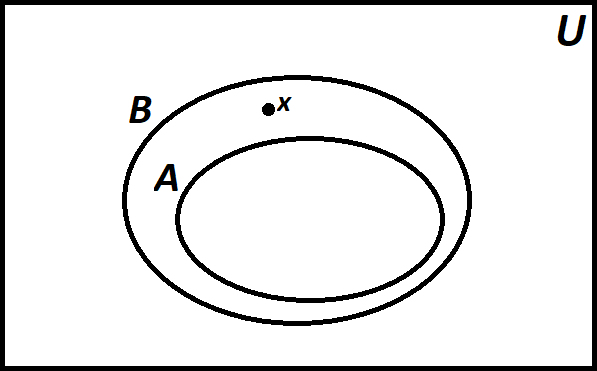
\includegraphics[width = 7 cm]{figures/sets/fig-sets-02-00.png}
      \caption{O conjunto $A$ está contido no conjunto $B$, equivalentemente, $B$ contém $A$.}
      \label{fig:sets-02-00}
  \end{figure}

  \textbf{Interseção:} Se estamos interessados em conjuntos/elementos que pertencem simultaneamente a dois conjuntos $A$ e $B$, dizemos que estamos interessados na interseção de $A$ e $B$ (denotada como $A \cap B$)$^{\ref{fig:sets-02-01}}$.

  \begin{figure}[hbt!]
      \centering
      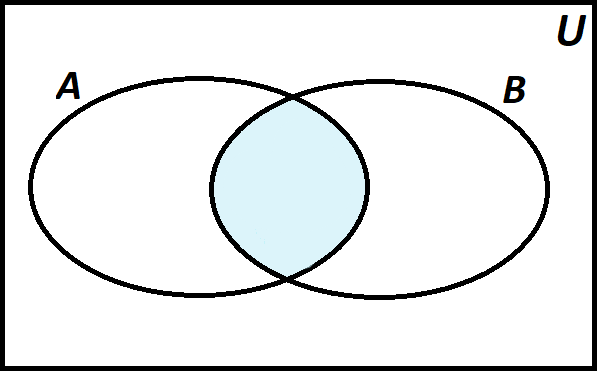
\includegraphics[width = 7 cm]{figures/sets/fig-sets-02-01.png}
      \caption{A região azul representa a visualização da interseção dos conjuntos $A$ e $B$.}
      \label{fig:sets-02-01}
  \end{figure}

  \textbf{União:} Já se estamos interessados nos conjuntos/elementos que fazem parte de $A$ ou de $B$ dizemos que, nosso objetivo é a união de $A$ e $B$ ($A \cup B$)$^{\ref{fig:sets-02-02}}$.

  \begin{figure}[hbt!]
      \centering
      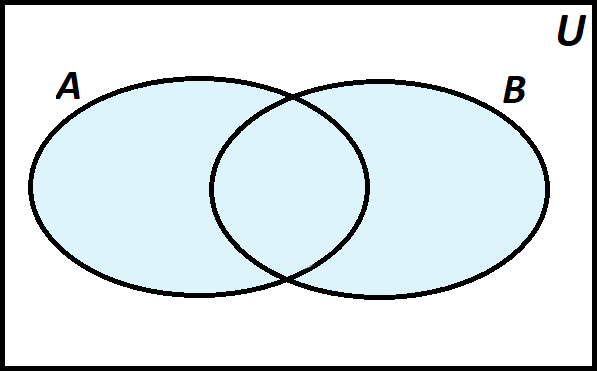
\includegraphics[width = 7 cm]{figures/sets/fig-sets-02-02.png}
      \caption{A região azul representa a visualização da união dos conjuntos $A$ e $B$.}
      \label{fig:sets-02-02}
  \end{figure}

  \textbf{Universo:} Quando estamos trabalhando com conjuntos é comum definirmos quem é nosso universo ($ \mathcal U $), isto é, o conjunto que conterá todos os conjuntos/elementos que estaremos trabalhando em um contexto$^{\ref{fig:sets-02-03}}$. Por exemplo, na reta real nosso universo é $\mathcal U = \mathbb{R}$.

  \begin{figure}[hbt!]
      \centering
      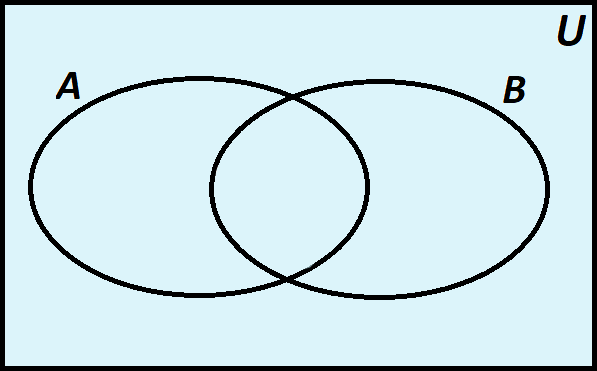
\includegraphics[width = 7 cm]{figures/sets/fig-sets-02-03.png}
      \caption{A região azul representa a visualização do nosso Universo.}
      \label{fig:sets-02-03}
  \end{figure}

  \textbf{Conjunto Complementar:} Sendo $A$ um conjunto, dizemos que o conjunto $A$ complementar ou complemento de $A$ (denotado como $\overline A$ ou $A^C$)contém todos os conjuntos/elementos que não estão contidos/pertencem a $A$, mas fazem parte de nosso universo ($\mathcal U$)$^{\ref{fig:sets-02-04}}$.

  \begin{figure}[hbt!]
      \centering
      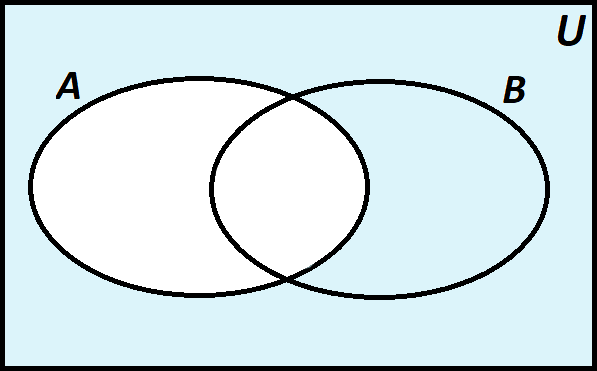
\includegraphics[width = 7 cm]{figures/sets/fig-sets-02-04.png}
      \caption{A região azul representa a visualização do complemento de $A$.}
      \label{fig:sets-02-04}
  \end{figure}

  \textbf{Diferença de Conjuntos :} Quando temos dois conjuntos e nosso objetivo são os conjuntos/elementos que pertencem a um destes conjuntos, mas não do outro dizemos que estamos interessados na diferença destes conjuntos. No caso, se quero os conjuntos/elementos de $B$, mas não queremos pegar os que também pertencem a $A$, queremos os elementos/conjuntos que pertencem a diferença de $B$ com $A$ (denotamos como $B-A$ ou $B \backslash A$)$^{\ref{fig:sets-02-05}}$.

  \begin{figure}[hbt!]
      \centering
      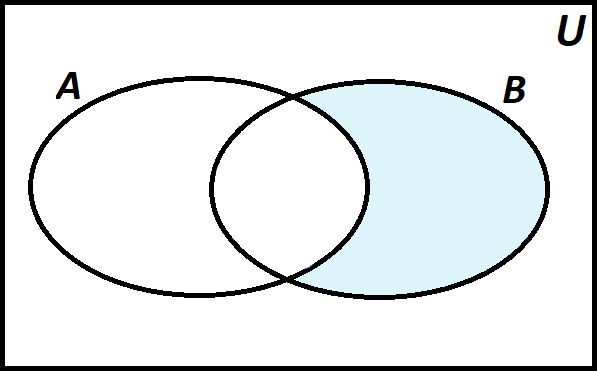
\includegraphics[width = 7 cm]{figures/sets/fig-sets-02-05.png}
      \caption{A região azul representa a visualização da diferença entre os conjuntos $B$ e $A$, isto é, a área onde estão os elementos que pertencem a $B$, mas não pertencem a $A$.}
      \label{fig:sets-02-05}
  \end{figure}

  Lembre-se: os diagramas apresentados servem como ferramenta auxiliar para ajudar a entender os conceitos, mas não devem ser vistos como a única ferramenta para compreender as definições e  a teoria exposta.

  \subsection{Definições}
  
  Seja $A$ e $B$ conjuntos quaisquers, $\mathcal{U}$ nosso universo e $\emptyset$ o conjunto vazio. Assim, temos formalmente (e em FOL):

  \begin{itemize}
    \item \textbf{Conjunto Vazio}: $\emptyset = \{x | false\}$
    
    \[\forall x (x \in \emptyset \iff \bot)\]
    
    \qquad
    
    \item \textbf{Universo}: $\mathbb{U} = \{x | true \}$
    
    \[\forall x (x \in \mathbb{U} \iff \top)\]
    
    \qquad
    
    \item \textbf{União}: $A \cup B = \{x | x \in A \vee x \in B\}$
    
    \[\forall x (x \in A \cup B \iff x \in A \vee x \in B)\]
    
    \qquad
    
    \item \textbf{Interseção}: $A \cap B = \{x | x \in A \wedge x \in B\}$
    
    \[\forall x (x \in A \cap B \iff x \in A \wedge x \in B)\]
    
    \qquad
    
    \item \textbf{Diferença}: $A \backslash B = \{x | x \in A \wedge x \notin B\}$
    
    \[\forall x (x \in A \backslash B \iff x \in A \wedge x \notin B)\]
    
    \qquad
    
    \item \textbf{Complementar}: $\overline A = \mathcal{U} \backslash A = \{x | x \in \mathcal{U} \land x \notin A\}$
    
    \[\forall x (x \in \overline A \iff x \notin A)\]
  \end{itemize} 

  \subsection{Axiomas}
  Agora iremos apresentar alguns axiomas que servirão como base para todo o desenvolvimento dos conteúdos aqui propostos. Quando utilizarmos a palavra elemento, estaremos utilizando-a com a ideia de que um conjunto que pertença a outro é um elemento do segundo, para evitar repetir o uso excessivo da palavra conjunto.

  \textbf{Axioma da Extensionalidade:} Dois conjuntos são iguais, se e somente se, todo elemento que pertence ao primeiro conjunto pertence ao segundo e todo elemento que pertence ao segundo também pertence ao primeiro, ou seja:

  \[\forall A \hspace{1.5mm} \forall B \hspace{1.5mm} (A = B) \iff (\forall x \hspace{1.5mm} (x \in A \iff x \in B))\]

  Através desse axioma fica mais claro de entender duas propriedades dos conjuntos.

  Deste axioma, vem a explicação do motivo de que a ordem dos elementos de um conjunto não importa. Pois dado dois conjuntos com os mesmos elementos, mas em ordem diferente (por exemplo, $X=\{a,b,c,d,e,f\}$ e o conjunto $Y=\{e,c,f,b,a,d\}$) eles ainda satisfazem a propriedade de que se $t$ pertence a um deles implica $t$ pertencer ao outro. Outro ponto interessante é que não importa se um conjunto possui elementos repetidos ele continuará igual ao que possui apenas um elemento, isto é, $X=\{a,b,d,e\}$ é igual ao $Y=\{b,a,d,a,e,b,b\}$. Ou seja, em um conjunto não importa a ordem e nem as repetições de elementos.

  \textbf{Axioma da Existencia do Conjunto Vazio: } Diremos que no nosso universo ($\mathbb{U}$), existe um conjunto tal que ele não contém ninguém, ou seja, ele é vazio, daí seu nome, Conjunto Vazio (denotado por $\emptyset$). O axioma é:

    \[\exists A \hspace{1.5mm} \forall x \hspace{1.5mm} \neg\hspace{0.5mm} (x \in A)\]

  \textbf{Unicidade do Conjunto Vazio}

  Podemos provar a unicidade do conjunto vazio a partir dos dois axiomas acimas, suponhamos que existam dois conjuntos ($A$ e $B$) com a propriedade do conjunto vazio, assim utilizando o axioma da Extensão concluíremos que eles são iguais, suponhamos $t$ arbitrário:

  \begin{center}
      \begin{landscape}
      \AxiomC{$\forall a  \forall b  (a = b) \iff (\forall x  (x \in a \iff x \in b))$}
      \UnaryInfC{$(A = B) \iff (\forall x  (x \in A \iff x \in B))$}
      \AxiomC{$t \in A $}
      \AxiomC{}
      \RightLabel{\scriptsize $1$}
      \UnaryInfC{$\forall x \neg (x \in A)$}
      \UnaryInfC{$\neg (t \in A)$}
      \BinaryInfC{$\perp$}
      \UnaryInfC{$t \in B$}
      \AxiomC{$t \in B$}
      \AxiomC{}
      \RightLabel{\scriptsize $1$}
      \UnaryInfC{$\forall x \neg (x \in B)$}
      \UnaryInfC{$\neg (t \in B)$}
      \BinaryInfC{$\perp$}
      \UnaryInfC{$t \in A$}
      \RightLabel{\scriptsize $\iff I_1$}
      \BinaryInfC{$t \in A \iff t \in B$}
      \UnaryInfC{$\forall x  (x \in A \iff x \in B)$}
      %\RightLabel{\scriptsize $\to E_4$}
      \BinaryInfC{A=B}
      \DisplayProof
      \end{landscape}
  \end{center}

  \textbf{Axioma do Par: } Este axioma nos diz que para todos os conjuntos $A$ e $B$, existe um conjunto conjunto que é $\{A,B\}$. Ou seja,

    \[\forall A \hspace{1.5mm} \forall B \hspace{1.5mm} \exists C \hspace{1.5mm} \forall x \hspace{1.5mm} (x \in C \leftrightarrow x = A \vee x = B)\]

  Vale ressaltar que se $A=B$, teremos $\{A,B\}=\{A,A\}=\{A\}$. A aplicação sucessiva deste axioma nos permite criar uma infinidade de conjuntos finitos. Por exemplo, $A=\emptyset$ e seja $B=\emptyset$, assim teremos $\{\emptyset\}$, sendo $B=\{\emptyset\}$, teremos agora $\{\emptyset,\{\emptyset\}\}$, agora fazendo $A=\{\emptyset\}$, teremos $\{\{\emptyset\}\}$.

  Não pretendemos nos aprofundar mais nos axiomas de conjuntos, dado que eles utilizarão conceitos abordados futuramente, nos capítulos de Relações, Funções e Axiomas.

  Mas como se pode ver em ..., podemos reduzir uma grande gama de coisas a conjuntas, assim podemos tratá-las na Teoria dos Conjuntos. Para saber mais sobre Teoria dos Conjuntos dê uma olhada em ... .

\section{Diagrama de Venn}
A maneira mais simples de entender a Teoria de Conjuntos, talvez seja o Diagrama de Venn. Criado por John Venn em 1880, esse sistema de representar graficamente conjuntos auxilia imensamente quem está começando a aprender esse assunto, principalmente para entender sobre a parte inicial de notações. Basicamente, consiste em representar num plano, o universo $\mathcal U$ como sendo um retângulo e cada conjunto $A,B,...$ como uma curva fechada simples (geralmente, círculo).

  \subsection{Para 1 ou 2 conjuntos}
  Começando com a ideia mais simples, a imagem abaixo representa em vermelho o conjunto $A$ dentro do universo $\mathcal U$:

  %\begin{figure}[h!]
  %    \centering
  %    \includegraphics{fig_set_01_01.png}
  %    \caption{Conjunto $A$ dentro de $\mathcal U$}
  %    \label{fig:fig_set_01_01}
  %\end{figure}

  Já sobre o conjunto complementar $A^c$, ele simplesmente é a parte que está no retângulo, mas não está no círculo, justamente o que não estava de vermelho na figura anterior.

  %\begin{figure}[h!]
  %    \centering
  %    \includegraphics{fig_set_01_02.png}
  %    \caption{Conjunto complementar $A^c$}
  %    \label{fig:fig_set_01_02}
  %\end{figure}

  Para representar que um elemento pertence ao conjunto $A$, simplesmente colocamos ele dentro do espaço delimitado pelo círculo que representa o conjunto, e para representar que um elemento nāo pertence ao conjunto $A$, fazemos o inverso.


  %\begin{figure}[h!]
  %    \centering
  %    \includegraphics{figure_set_01_03.png}
  %    \caption{$a \in A$ e $b \notin A$}
  %    \label{fig:figure_set_01_03}
  %\end{figure}

  Quando vamos representar mais de um conjunto em um diagrama de Venn, devemos necessariamente ter todas as possíveis relações, mas o que isso significa? Por exemplo, quando temos $2$ conjuntos $A$ e $B$, significa que devemos ter $4$ regiões representando respectivamente: elementos que pertencem somente à $A$, elementos que pertencem somente à $B$, elementos que pertencem à $A$ e à $B$ simultaneamente e elementos que não pertencem a nenhum dos conjuntos. Precisamos disso, para que tudo que provarmos para dois conjuntos $A$ e $B$, possa ser generalizado para dois conjuntos quaisquer, independente do problema e da situação que estamos estudando.

  Utilizando esse artífiico, podemos representar todas as definições de intersecçāo, uniāo e diferença de $2$ conjuntos, introduzidas na seçāo anterior. Veja nas figuras abaixo:

  %\begin{figure}[h!]
  %    \centering
  %    \includegraphics{figure_set_01_04.png}
  %    \caption{Intersecção $A \cap B$}
  %    \label{fig:figure_set_01_04}
  %\end{figure}

  %\begin{figure}[h!]
  %    \centering
  %    \includegraphics{figure_set_01_05.png}
  %    \caption{União $A \cup B$}
  %    \label{fig:figure_set_01_05}
  %\end{figure}

  %\begin{figure}[h!]
  %    \centering
  %    \includegraphics{figure_set_01_06.png}
  %    \caption{Diferença $A \setminus B$}
  %    \label{fig:figure_set_01_06}
  %\end{figure}

  Todavia, isso ainda não permite fazer tudo que desejamos. Se quisermos representar que $A \subseteq B$, a ideia inicial seria colocar o círculo $A$ dentro do círculo $B$, quebrando o rigor de manter todas as possíveis relações, pois não teremos uma região para representar os elementos que pertecem somente a $A$. Então, como resolver esse problema? Representamos os conjuntos $A$ e $B$ da mesma forma que anteriormente e também escrevemos o símbolo do conjunto vazio $\emptyset$ na região dos elementos que pertencem somente a $A$. Assim, só existem elementos no conjunto $A$ que estão na região $A\cap B$, ou seja, se um elemento está em $A$, como consequência ele está em $B$, exatamente a definição de $A \subseteq B$.

  %\begin{figure}[h!]
  %    \centering
  %    \includegraphics{figure_set_01_07.png}
  %    \caption{Subconjunto $A \subseteq B$}
  %    \label{fig:figure_set_01_07}
  %\end{figure}

  É inegável que para muitos exemplos isso se torna inviável, principalmente quando o único objetivo é fazer uma ilustração matemática do problema, como por exemplo: tomamos o universo $\mathcal U$ como a fauna do nosso planeta, nele temos dois conjuntos $A$ de humanos e $B$ de mamíferos. É previamente conhecido que todos os humanos são mamíferos, falando de outra forma, que $A \subseteq B$. Logo, pra representar um problema que envolva esses elementos, podemos utilizar o \textbf{Diagrama de Euler}, similar ao Diagrama de Venn, com a diferença de que não é necessário mostrar todas as possíveis relações, mas apenas as relações específicas do problema retratado. E assim, fazemos exatamente o que tinha sido proposto no parágrafo anterior e, colocar o círculo $A$ dentro do círculo $B$.

  %\begin{figure}[h!]
  %    \centering
  %    \includegraphics{figure_set_01_08.png}
  %    \caption{Diagrama de Euler $A \subseteq B$}
  %    \label{fig:figure_set_01_08}
  %\end{figure}

  \subsection{Para 3 conjuntos ou mais}
  Já foi bastante falado sobre Diagrama de Venn, mas nem chegamos a trabalhar com mais de $2$ conjuntos, o que é importante, dado que a Teoria de Conjuntos não se resume a $A$ e $B$. Mas antes de partirmos para mais conjuntos, vamos pensar numa generalização de quantas regiões diferentes devemos ter para que o diagrama seja um Diagrama de Venn. Dado $n$ conjuntos diferentes, tomamos um elemento qualquer $x$, e para cada um dos $n$ conjuntos existem duas possibilidades: $x \in $ conjunto e $x \notin $ conjunto. Logo, concluímos que existem $\underbrace{\begin{matrix} 2\cdot2\cdots2\cdot2\end{matrix}}_{n} = 2^n$ possibilidades de pertencimento de $x$ nos conjuntos, equivalente à dizer que existem $2^n$ regiões diferentes. Isso bate perfeitamente com o caso anterior pra $2$ conjuntos, pois vimos que era necessário ter $4=2^2$ regiões diferentes.

  Agora, com $3$ conjuntos $A$, $B$ e $C$, o número de regiões diferentes é $2^3=8$, mas como iremos representá-las? A primeira ideia que vem a cabeça é adicionar um círculo representando o conjunto $C$ no diagrama da figura $\ref{fig:sets-02-00}$, intersectando as regiões já existentes, resultando na figura abaixo:

  Fazendo uma rápida contagem, obtemos $8$ regiões diferentes, exatamente como deve ser (lembrete: A região fora dos conjuntos mas dentro do universo $\mathcal U$, também é considerada na contagem). E da mesma forma que representamos intersecção, união e diferença de conjuntos anteriormente, também podemos representar com $3$ conjuntos, veja abaixo:

  %\begin{figure}[h!]
  %    \centering
  %    \includegraphics{figure_set_01_09.png}
  %    \caption{Intersecção $A \cap B \cap C$}
  %    \label{fig:figure_set_01_09}
  %\end{figure}

  %\begin{figure}[h!]
  %    \centering
  %    \includegraphics{figure_set_01_10.png}
  %    \caption{União $A \cup B \cup C$}
  %    \label{fig:figure_set_01_10}
  %\end{figure}

  %\begin{figure}[h!]
  %    \centering
  %    \includegraphics{figure_set_01_11.png}
  %    \caption{Diferença $A \setminus (B \cup C)$}
  %    \label{fig:figure_set_01_11}
  %\end{figure}

  Sendo ganancioso e indo além, podemos querer representar $4$ conjuntos, adicionando o conjunto $D$. E igual o caso anterior, só temos que adicionar mais um círculo representando o conjunto $D$ e, dado que antes obtemos um triângulo de círculos, dessa vez iremos ter uma quadrado de cícurlos, correto?

  \textbf{ERRADO!} Se você é um leitor observador, já deve ter notado que esse diagrama não possui as $2^4=16$ regiões diferentes necessárias, mas somente $14$. Não existem regiões que representam os elementos que pertencem ao mesmo tempo aos conjuntos $A$ e $D$, mas não pertencem ao conjunto $B$ e nem ao $C$, e o inverso disso, ou seja, os elementos que pertencem ao mesmo tempo aos conjuntos $B$ e $C$, mas não pertencem ao conjunto $A$ e nem ao $D$.

  É válido ressaltar que é impóssível utilizar $4$ círculos pra representar $4$ conjuntos em um diagrama de Venn. Contudo, existem diagramas de Venn pra $4$ conjuntos, e antes de ler o próximo parágrafo, pegue uma folha e tente encontrar possíveis maneiras dessa representação. Dica: Não se abstenha de utilizar formas bem diferenciadas.

  Se você conseguiu, parabéns. Saiba que existem diversas maneiras, como por exemplo: $4$ elipses ou $3$ círculos e uma forma semelhante à metade de uma rosquinha. Fique a vontade para pesquisar na internet essas e outras maneiras de representação. Ainda assim, é relevante mostrar pelo menos uma delas, e escolhemos a da figura abaixo, muito semelhante a dois corações.

  %\begin{figure}[h!]
  %    \centering
  %    \includegraphics{figure_set_01_11.png}
  %    \caption{Diagrama de Venn para 4 conjuntos}
  %    \label{fig:figure_set_01_11}
  %\end{figure}

  Podemos continuar e encontrar representações para $5$ ou mais conjuntos, as quais vão ficando cada vez mais complicadas. Porém, como nosso principal objetivo é utilizar visualizações gráficas para facilitar o aprendizado em Teoria de Conjuntos, a partir do momento que isso vem a se tornar complicado, perde totalmente a utilidade. Por esse motivo, vamos parar em $4$ conjuntos, mas se a curiosidade for grande, procure aprender mais sobre esse assunto.

  \subsection{Aplicações}
  A mais importante e útil das aplicações é justamente demonstrar propriedades da Teoria de Conjuntos. Se fosse solicitado para você leitor demonstrar as propriedades a seguir, somente com o que aprendeu até agora, já conseguiria utilizar o Diagrama de Venn para demonstrá-las. Apesar de parecer complicado, é incrivelmente simples, veja:

  \textbf{Exemplo 1:} Demonstre que $A \setminus B = A \cap B^c$.

  \textbf{Resposta:} Primeiramente, vamos fazer o Diagrama de Venn desses dois conjuntos e enumerar as $4$ regiões:

  %\begin{figure}[h!]
  %    \centering
  %    \includegraphics{figure_set_01_12.png}
  %    \caption{Regiões 1, 2, 3 e 4}
  %    \label{fig:figure_set_01_12}
  %\end{figure}

  Assim, temos que $A=\{1,2\}$, $B=\{2,3\}$, $A^c=\{3,4\}$ e $B^c=\{1,4\}$. Utilizando esse valores, podemos calcular $A \setminus B$ e $A \cap B^c$, conforme abaixo:

  \begin{equation*}
    \begin{aligned}
      A \setminus B &= \{1,2\} \setminus \{2,3\} = \{1\}\\
      A \cap B^c &= \{1,2\} \cap \{1,4\} = \{1\}
    \end{aligned}
  \end{equation*}

  Portanto, concluímos que $A \setminus B = A \cap B^c$.

  \textbf{Exemplo 2:} Demonstre que $(A \setminus B) \cup (B \setminus A) = (A \cup B) \setminus (A \cap B)$.

  \textbf{Resposta:} Utilizando o mesmo Diagrama de Venn e a mesma numeração de regiões do exemplo anterior, temos:

  \begin{equation*}
    \begin{aligned}
      A \setminus B &= \{1,2\} \setminus \{2,3\} = \{1\}\\
      B \setminus A &= \{2,3\} \setminus \{1,2\} = \{3\}\\
      A \cup B &= \{1,2\} \cup \{2,3\} = \{1,2,3\}\\
      A \cap B &= \{1,2\} \cap \{2,3\} = \{2\}\\
      (A \setminus B) \cup (B \setminus A) &= \{1\} \cup \{3\} = \{1,3\}\\
      (A \cup B) \setminus (A \cap B) &= \{1,2,3\} \setminus \{2\} = \{1,3\}
    \end{aligned}
  \end{equation*}

  Portanto, concluímos que $(A \setminus B) \cup (B \setminus A) = (A \cup B) \setminus (A \cap B)$.
  \newline
  É possível responder essas questões somente utilizando o diagrama e pintando as regiões, mas a enumeração torna o processo mais fácil.

  $\qquad$

  Outra aplicação interessante, muito recorrente em testes de lógica e vestibulares, é tentar interpretar problemas da vida real com conjuntos, conforme no exemplo a seguir.

  \textbf{Exemplo 3:} Em uma sala de aula do Ensino Fundamental com $40$ alunos, a professora Ana perguntou quem gostava de matemática e quem gostava de português. Ela obteve os seguintes dados:

  \begin{itemize}
    \item $21$ alunos gostam de matemática
    \item $17$ alunos gostam de português
    \item $9$ alunos não gostam de nenhuma das matérias
  \end{itemize}

  Quantos alunos gostam de ambas as matérias?

  \textbf{Resposta:} Vamos utilizar um Diagrama de Venn para dois conjuntos, onde um conjunto representa os alunos que gostam de matemática e o outro representa os que gostam de português.
  Dado que $9$ alunos não gostam de nenhuma das matérias e temos $40$ alunos na sala, então $40-9=31$ alunos pertencem a pelo menos um dos conjuntos, ou seja, gostam de matemática ou português.

  Como $21$ gostam de matemática, logo $31-21=10$ gostam somente de português (região da esquerda) e, analogamente, como $17$ gostam de português, logo $31-17=14$ gostam somente de matemática (região da direita). Utilizando esses dados, vemos que ainda faltam $31-10-14=7$ alunos, justamente os que gostam de ambas as matérias (região do meio). Veja abaixo o diagrama final:

  %\begin{figure}[h!]
  %    \centering
  %    \includegraphics{figure_set_01_13.png}
  %    \caption{Diagrama de Venn para Matemática e Português}
  %    \label{fig:figure_set_01_13}
  %\end{figure}

  $\qquad$

  Apesar do estudo de conjuntos com Diagrama de Venn ser fácil, simples e útil, como já comentado anteriormente, é difícil para trabalhar com muitos conjuntos, além das provas utilizando esse recurso não terem um grau de formalidade muitas vezes requerido pelos matemáticos. Devido a esse fato, iremos estudar nas próximas seções outras maneiras de lidar com Teoria dos Conjuntos, como provas matemáticas formais, dedução natural, cálculo em conjuntos e é claro, utilizando o Lean.

\section{Prova de Teoremas}
Nesta seção iremos tratar de formalizar definições e Teoremas. Ao contrário da seção $5.2$, onde o foco era transmitir a notação e uma ideia geral dos conceitos.

Aqui serão apresentadas algumas provas em Lean para o conteúdo apresentado. Não se preocupe, caso não entenda sobre o que o código quer dizer ignore ele por enquanto e após ler as próximas duas seções (que falam de conjuntos em Lean), volte e tente compreender o que foi feito. Já que o foco principal nesta parte são as provas matemáticas tradicionais e as definições mais precisas.

  \subsection{Prova Matemática Formal}
  Ainda vai ter algo escrito aqui

  \subsection{Dedução Natural}
  Ainda vai ter algo escrito aqui

\section{Conjuntos em Lean}
Embora na teoria axiomática dos conjuntos se considere conjuntos de objetos distintos, em matemática é mais comum considerar subconjuntos de algum dominio fixo ($\mathcal U $). É assim que os conjuntos são tratados em Lean. Para qualquer dado do tipo $U$, Lean nos retorna um novo dado tipo $conjunto$ $U$, que consiste no conjunto dos elementos de $U$. Assim, por exemplo, podemos raciocinar sobre conjuntos de números naturais, conjuntos de números inteiro ou conjuntos de pares de números naturais.

  \subsection{Notações}
  O lean possui uma biblioteca padrão para lidar com conjuntos chamada set e, sempre que formos utilizar um comando que pertence à ela, é necessário escrever {\fontencoding{U}\fontfamily{cmtt}\selectfont set.comando}. Entretanto, pra facilitar nossa vida, podemos escrever {\fontencoding{U}\fontfamily{cmtt}\selectfont open set} no início do código, o que permite escrevermos somente {\fontencoding{U}\fontfamily{cmtt}\selectfont comando}, e o lean já entende que ele pertence a biblioteca set.

  Além disso, para trabalharmos com conjuntos, também é essencial definirmos um tipo {\fontencoding{U}\fontfamily{cmtt}\selectfont U} e sabermos utilizar conjuntos e elementos desse tipo. Para isso, utilizamos o código abaixo:

  \begin{lstlisting}
  open set

  variable {U : Type}
  variables A B C : set U
  variable x : U \end{lstlisting}

  Temos aqui uma pequena lista de como se representa os principais caractéres da parte de conjuntos em Lean:

  \begin{itemize}
      \item $\in$ $\rightarrow$ $\backslash$in

      \item $\notin$ $\rightarrow$ $\backslash$notin

      \item $\subset$ $\rightarrow$ $\backslash$subset

      \item $\subseteq$ $\rightarrow$ $\backslash$sub

      \item $\emptyset$ $\rightarrow$ $\backslash$empty

      \item $\cup$ $\rightarrow$ $\backslash$un \ ou \ $\backslash$cup \ ou \ $\backslash$union

      \item $\cap$ $\rightarrow$ $\backslash$i \ ou \ $\backslash$cap \ ou \ $\backslash$intersection
  \end{itemize}

  Obs$^{1}$.: O conjunto universal é denotado {\fontencoding{U}\fontfamily{cmtt} \selectfont univ}.

  Obs$^{2}$.: O complementar de um conjunto é denotado com um símbolo de negação antes de seu símbolo, assim: $-A$

  Podemos ver alguns exemplos abaixo:
  \begin{lstlisting}
    open set
    variable {U : Type}
    variables A B C : set U
    variable x : U

    #check x ∈ A
    #check A ∪ B
    #check B \ C
    #check C ∩ A
    #check -C
    #check ∅ ⊆ A
    #check B ⊆ univ \end{lstlisting}

  Noções básicas da teoria dos conjuntos são definidas na biblioteca principal do Lean, mas teoremas e notações adicionais que iremos utilizar nesse capítulo, estão disponíveis em uma biblioteca auxiliar que é carregada com o comando
  {\fontencoding{U}\fontfamily{cmtt} \selectfont import data.set}, o qual deve aparecer no início do arquivo.

  \begin{lstlisting}
    import data.set
    open set
    variable {U : Type}
    variables A B C : set U
    variable x : U \end{lstlisting}

  A partir desse momento, para evitar repetição, iremos omitir as $4$ primeiras linhas do código, no entanto \textbf{você deve lembrar que elas existem para seu código funcionar.} Já sobre a linha $5$, não é necessário escrever nos próximos exemplos, pois sempre iremos se referenciar a um elemento do tipo{\fontencoding{U}\fontfamily{cmtt} \selectfont U}, dentro de {\fontencoding{U}\fontfamily{cmtt}\selectfont example, lemma} ou {\fontencoding{U}\fontfamily{cmtt}\selectfont theorem}.

  \subsection{Primeiros Passos}

  Relembrando a definição de subconjunto, podemos utilizar o template abaixo para mostrar que o conjunto $A$ é um subconjunto de $B$:

  \begin{lstlisting}
  example : A ⊆ B :=
  assume x : U,
  assume h : x ∈ A,
  show x ∈ B, from sorry \end{lstlisting}

  Obs: Na linha $2$ poderíamos ter escrito somente {\fontencoding{U}\fontfamily{cmtt}\selectfont assume x}, pois já inferiria que {\fontencoding{U}\fontfamily{cmtt}\selectfont x} é do tipo {\fontencoding{U}\fontfamily{cmtt}\selectfont U}.

  Já para mostrar que $A$ e $B$ são iguais, temos dois comandos diferentes: {\fontencoding{U}\fontfamily{cmtt}\selectfont eq\_of\_subset\_of\_subset} e {\fontencoding{U}\fontfamily{cmtt}\selectfont ext}.

  \textbf{eq\_of\_subset\_of\_subset:} Ele funciona interpretando a seguinte expressão $(A \subseteq B \wedge B \subseteq A) \Rightarrow A=B$, ou seja, obtém a equivalência dos conjuntos a partir do fato de que o primeiro é subconjunto do segundo, e vice-vera. Veja o código:

  \begin{lstlisting}
  example : A = B :=
  eq_of_subset_of_subset
    (assume x,
      assume h : x ∈ A,
      show x ∈ B, from sorry)
    (assume x,
      assume h : x ∈ B,
      show x ∈ A, from sorry) \end{lstlisting}

  \textbf{ext:} É uma sigla para ``extensionality", ou seja, extensionalidade. Matemáticamente, isso representa a expressão $\forall x \ (x \in A \leftrightarrow x \in B) \Rightarrow A=B$. Veja o código:

  \begin{lstlisting}
  example : A = B :=
  ext (assume x, iff.intro
    (assume h : x ∈ A,
      show x ∈ B, from sorry)
    (assume h : x ∈ B,
      show x ∈ A, from sorry)) \end{lstlisting}

  Além disso, o Lean possui interpretação ambígua para regras de união, interseção e outras operações em conjuntos que são consideradas “definições”. Isso significa que as expressões $x$ $\in$ $A$ $\cap$ $B$ e $x$ $\in$ $A$ $\wedge$ $x$ $\in$ $B$ possuem a mesma interpretação no Lean. Isso também é válido para outras construções em conjuntos, como: $x$ $\in$ $A$ $\backslash $ $B$ e $x$ $\in$ $A$ $\wedge$ $\neg$ $(x$ $\in$ $B)$. O termo $\neg$ $(x$ $\in$ $B)$ é somente outra forma de escrever $x$ $\notin$ $B$. Abaixo são apresentadas algumas aplicações dessa interpretação:

  \begin{lstlisting}
  example : ∀ x, x ∈ A → x ∈ B → x ∈ A ∩ B :=
  assume x,
  assume h₁ : x ∈ A,
  assume h₂ : x ∈ B,
  show x ∈ A ∩ B, from and.intro h₁ h₂

  example : A ⊆ A ∪ B :=
  assume x,
  assume h : x ∈ A,
  show x ∈ A ∪ B, from or.inl h

  example : ∅ ⊆ A  :=
  assume x,
  assume h : x ∈ (∅ : set U),
  show x ∈ A, from false.elim h \end{lstlisting}

  Observe no último exemplo a necessidade de usar a notação {\fontencoding{U}\fontfamily{cmtt} \selectfont ($\emptyset$ : set U)}, dizendo ao nosso provador que o $\emptyset$ é um conjunto de {\fontencoding{U}\fontfamily{cmtt}
  \selectfont U}. Isso acontece pois ele não consegue inferir que tipo é o conjunto vazio, dado que por definição, esse conjunto existe em qualquer universo, ou seja, pode ser de qualquer tipo.

  Opcionalmente, podemos usar alguns teoremas da biblioteca {\fontencoding{U}\fontfamily{cmtt}
  \selectfont data.set}, projetados especificamente para uso em conjuntos:

  \begin{lstlisting}
  example : ∀ x, x ∈ A → x ∈ B → x ∈ A ∩ B :=
  assume x,
  assume : x ∈ A,
  assume : x ∈ B,
  show x ∈ A ∩ B, from mem_inter ‹x ∈ A› ‹x ∈ B›

  example : A ⊆ A ∪ B :=
  assume x,
  assume h : x ∈ A,
  show x ∈ A ∪ B, from mem_union_left B h

  example : ∅ ⊆ A  :=
  assume x,
  assume : x ∈ ∅,
  show x ∈ A, from absurd this (not_mem_empty x) \end{lstlisting}

  Lembre-se que o comando{\fontencoding{U}\fontfamily{cmtt}
  \selectfont absurd} pode ser usado para provar qualquer fato a partir de duas hipóteses contrárias: $h_1$ : $P$ e $h_2$ : $\neg$ $P$.

  Aqui, o teorema {\fontencoding{U}\fontfamily{cmtt}
  \selectfont not\_mem\_empty x} significa $x$ $\notin$ $\emptyset$. Para ver a declaração de teoremas disponíveis, utilize o comando{\fontencoding{U}\fontfamily{cmtt}
  \selectfont \#check}:

  \begin{lstlisting}
  #check @mem_inter
  #check @mem_of_mem_inter_left
  #check @mem_of_mem_inter_right
  #check @mem_union_left
  #check @mem_union_right
  #check @mem_or_mem_of_mem_union
  #check @not_mem_empty \end{lstlisting}

  Neste caso, o símbolo{\fontencoding{U}\fontfamily{cmtt}
  \selectfont @} impede que ele tente preencher argumentos implícitos automaticamente, forçando-o a exibir a declaração completa do teorema.

  Já que podemos relacionar conjuntos com suas definições lógica, isso auxilia a comprovação de inclusões entre conjuntos:

  \begin{lstlisting}
  example : A \ B ⊆ A :=
  assume x,
  assume : x ∈ A \ B,
  show x ∈ A, from and.left this

  example : A \ B ⊆ -B :=
  assume x,
  assume : x ∈ A \ B,
  have x ∉ B, from and.right this,
  show x ∈ -B, from this \end{lstlisting}

  Novamente, é possível usar versões dos teoremas projetados especificamente para conjuntos:

  \begin{lstlisting}
  example : A \ B ⊆ A :=
  assume x,
  assume : x ∈ A \ B,
  show x ∈ A, from mem_of_mem_diff this

  example : A \ B ⊆ -B :=
  assume x,
  assume : x ∈ A \ B,
  have x ∉ B, from not_mem_of_mem_diff this,
  show x ∈ -B, from this \end{lstlisting}

  Como o Lean tem que desenvolver definições, ele pode acabar se confundindo às vezes. Por exemplo, na prova a seguir, se você subtituir a última linha por {\fontencoding{U}\fontfamily{cmtt}\selectfont sorry}, ele terá problemas tentando entender que você quer que ele desenvolva o símbolo de subconjunto:

  \begin{lstlisting}
  example : A ∩ B ⊆ B ∩ A :=
  assume x,
  assume h : x ∈ A ∩ B,
  have h₁ : x ∈ A, from and.left h,
  have h₂ : x ∈ B, from and.right h,
  and.intro h₂ h₁ \end{lstlisting}

  Uma solução alternativa é usar o comando {\fontencoding{U}\fontfamily{cmtt}\selectfont show}. Na maioria das vezes, fornecer informações adicionais para o Lean pode ser útil. Outra solução é nomear um teorema, o que leva o Lean a usar um método um pouco diferente de processar a prova, corrigindo o problema como um efeito colateral de sorte.

  \begin{lstlisting}
  example : A ∩ B ⊆ B ∩ A :=
  assume x,
  assume h : x ∈ A ∩ B,
  have h₁ : x ∈ A, from and.left h,
  have h₂ : x ∈ B, from and.right h,
  show x ∈ B ∩ A, from sorry

  theorem my_example : A ∩ B ⊆ B ∩ A :=
  assume x,
  assume h : x ∈ A ∩ B,
  have h₁ : x ∈ A, from and.left h,
  have h₂ : x ∈ B, from and.right h,
  sorry \end{lstlisting}

\section{Propriedades}
A seguir teremos algumas propriedades e a prova do porque estão corretas.

  \subsection{Básicas}
  \begin{itemize}
  \item $A \cap A = A$
  \item $A \cup A = A$
  \item $A \cap \mathcal U = A$
  \item $A \cup \mathcal U = \mathcal U$
  \item $A \cap \emptyset = \emptyset$
  \item $A \cup \emptyset = A$
  \end{itemize}

  \subsection{Comutatividade}
  \begin{itemize}
  \item $A \cap B = B \cap A$
  \item $A \cup B = B \cup A$
  \end{itemize}

  \subsection{Associatividade}
  \begin{itemize}
  \item $(A \cap B) \cap C = A \cap (B \cap C)$
  \item $(A \cup B) \cup C = A \cup (B \cup C)$
  \end{itemize}

  \subsection{Distributividade}
  \begin{itemize}
  \item $A \cap (B \cup C) = (A \cap B) \cup (A \cap C)$
  \item $A \cup (B \cap C) = (A \cup B) \cap (A \cup C)$

\textbf{Prova em Lean:}
\begin{lstlisting}
import data.set
open set

variable U : Type
variables A B C : set U

example : A ∪ (B ∩ C) = (A ∪ B) ∩ (A ∪ C) :=
eq_of_subset_of_subset
    (assume x,
    assume h : x ∈ A ∪ (B ∩ C),
    or.elim h
        (assume h₁ : x ∈ A,
        have h₂ : x ∈ A ∪ B, from or.inl h₁,
        have h₃ : x ∈ A ∪ C, from or.inl h₁,
        show x ∈ (A ∪ B) ∩ (A ∪ C), from and.intro h₂ h₃)
        (assume h₁ : x ∈ B ∩ C,
        have h₂ : x ∈ B, from and.left h₁,
        have h₃ : x ∈ C, from and.right h₁,
        have h₄ : x ∈ A ∪ B, from or.inr h₂,
        have h₅ : x ∈ A ∪ C, from or.inr h₃,
        show x ∈ (A ∪ B) ∩ (A ∪ C), from and.intro h₄ h₅))
    (assume x,
    assume h : x ∈ (A ∪ B) ∩ (A ∪ C),
    have h₁ : x ∈ A ∪ B, from and.left h,
    have h₂ : x ∈ A ∪ C, from and.right h,
    or.elim h₁
        (assume h₃ : x ∈ A,
        show x ∈ A ∪ (B ∩ C), from or.inl h₃)
        (assume h₃ : x ∈ B,
        or.elim h₂
            (assume h₄ : x ∈ A,
            show x ∈ A ∪ (B ∩ C), from or.inl h₄)
            (assume h₄ : x ∈ C,
            have h₅ : x ∈ B ∩ C, from and.intro h₃ h₄,
            show x ∈ A ∪ (B ∩ C), from or.inr h₅))) \end{lstlisting}

  \end{itemize}

  \subsection{Complementar/Lei de Demorgan}
  \begin{itemize}
  \item $\mathcal U ^c = \emptyset$
  \item $\emptyset ^c = \mathcal U$
  \item $A \cap A^c = \emptyset$

  $(i)$ Provaremos que $ \forall x (x \in A \cap \overline A) \rightarrow \forall x  (x \in \emptyset) $ :

  \begin{center}
    \AxiomC{}
    \RightLabel{\scriptsize $1$}
    \UnaryInfC{$ \forall x (x \in A \cap \overline A)$}
    \UnaryInfC{$t \in A \cap \overline A$}
    \UnaryInfC{$t \in A \land t \in \overline A $}
    \UnaryInfC{$t \in A $}
    \AxiomC{}
    \RightLabel{\scriptsize $1$}
    \UnaryInfC{$ \forall x (x \in A \cap \overline A)$}
    \UnaryInfC{$t \in A \cap \overline A$}
    \UnaryInfC{$t \in A \land t \in \overline A $}
    \UnaryInfC{$t \in \overline A $}
    \UnaryInfC{$t \in \mathbb{U} \land t \notin A $}
    \UnaryInfC{$t \notin A $}
    \BinaryInfC{$\perp$}
    \UnaryInfC{$t \in \emptyset$}
    \UnaryInfC{$\forall x  (x \in \emptyset)$}
    \RightLabel{\scriptsize $1$}
    \UnaryInfC{$ \forall x (x \in A \cap \overline A) \rightarrow \forall x  (x \in \emptyset) $}
    \DisplayProof
  \end{center}

  $(ii)$ Provaremos que $ \forall x  (x \in \emptyset) \rightarrow \forall x (x \in A \cap \overline A)$ :
  \begin{center}
    \AxiomC{}
    \RightLabel{\scriptsize $1$}
    \UnaryInfC{$\forall x  (x \in \emptyset)$}
    \UnaryInfC{$\perp$}
    \UnaryInfC{$t \in A \cap \overline A$}
    \UnaryInfC{$ \forall x (x \in A \cap \overline A)$}
    \RightLabel{\scriptsize $1$}
    \UnaryInfC{$\forall x  (x \in \emptyset) \rightarrow \forall x (x \in A \cap \overline A)$}
    \DisplayProof
  \end{center}

  Portanto, de $(i)$ e $(ii)$, concluímos que $ \forall x (x \in A \cap \overline A) \iff \forall x  (x \in \emptyset) $, ou seja, $A \cap \overline A$.

  \item $A \cup A^c = \mathcal U$

  \textbf{Prova:}  Seja $x$ um elemento de $A \cup \overline A$, assim temos que
  \[x \in (A \cup \overline A)\]
  \[ \iff x \in A \vee x \in \overline A\]

  \item $(A^c)^c = A$
  \item $(A \cap B)^c = A^c \cup B^c$
  \item $(A \cup B)^c = A^c \cap B^c$
  \end{itemize}

  \subsection{Lei da Absorção}
  \begin{itemize}
  \item $A \cap (A \cup B) = A$

  \begin{lstlisting}
    lemma inter_subseq (H : Type)(P Q : set H) : P ∩ (P ∪ Q) = P :=
    eq_of_subset_of_subset
      (assume x,
        assume h : x ∈ P ∩ (P ∪ Q),
        show x ∈ P, from h.left)
      (assume x,
        assume h : x ∈ P,
        have h₁ : x ∈ P ∪ Q, from or.inl h,
        show x ∈ P ∩ (P ∪ Q), from and.intro h h₁)\end{lstlisting}

  \item $A \cup (A \cap B) = A$
  \end{itemize}

  \subsection{Extras}
  \begin{itemize}
  \item $A \setminus B = A \cap B^c$
  \end{itemize}

\section{Cálculo em Conjuntos}
Podemos provar que dois conjuntos são iguais argumentando sobre seus elementos, ou podemos ser mais eficientes e utilizar o cálculo juntamente com as propriedades vistas na seção $5.6$. Veja alguns exemplos:

  \textbf{Exemplo 1:} Demonstre que $(A \setminus B)^c = A^c \cup B$

  \textbf{Prova:} Expressamos o cálculo:
  \begin{equation*}
    \begin{aligned}
      (A \setminus B)^c &= (A \cap B^c)^c)\\
      &= A^c \cup (B^c)^c\\
      & = A^c \cup B
    \end{aligned}
  \end{equation*}

  $\qquad$

  Relembrando um dos exemplos da seção $5.3$:

  \textbf{Exemplo 2:} Demonstre que $(A \setminus B) \cup (B \setminus A) = (A \cup B) \setminus (A \cap B)$

  \textbf{Prova:} Novamente, o cálculo:
  \begin{equation*}
    \begin{aligned}
      (A \setminus B) \cup (B \setminus A) &= (A \cap B^c) \cup (B \cap A^c)\\
      &= ((A \cap B^c) \cup B) \cap ((A \cap B^c) \cup A^c)\\
      &= ((A \cup B) \cap (B^c \cup B)) \cap ((A \cup A^c) \cap (B^c \cup A^c))\\
      &= ((A \cup B) \cap \mathcal U) \cap (\mathcal U \cap (B^c \cup A^c))\\
      &= (A \cup B) \cap (B^c \cup A^c)\\
      &= (A \cup B) \cap (A^c \cup B^c)\\
      &= (A \cup B) \cap (A \cap B)^c\\
      &= (A \cup B) \setminus (A \cap B)
    \end{aligned}
  \end{equation*}

Esses são exemplos simples de prova de teoremas sobre conjuntos com uso de cálculo; no entanto, podemos desejar realizar provas mais longas, com verificação. Felizmente, Lean ofereçe uma gama de axiomas sobre conjuntos que permitem desenvolver cálculos desse tipo, através do modo Cáculo.

Nos próximos exemplos, omitomos as quatro primeiras linhas, no entanto, lembre-se que elas existem, e devem ser incluídas no uso do provador.

\begin{lstlisting}
    import data.set
    open set
    variable U : Type
    variables A B C : set U

    example (h : A = B) : B = A :=
      calc
        B = A : eq.symm h
\end{lstlisting}

Nesse caso, utilizamos {\fontencoding{U}\fontfamily{cmtt}\selectfont eq.symm h}, que já nos deu a igualdade {\fontencoding{U}\fontfamily{cmtt}\selectfont B = A} direto. Mas tem outro jeito. Podemos querer somente baseado em {\fontencoding{U}\fontfamily{cmtt}\selectfont h}, reescrever {\fontencoding{U}\fontfamily{cmtt}\selectfont B}, e para isso utilizamos a tática {\fontencoding{U}\fontfamily{cmtt}\selectfont rewrite}.

  \begin{lstlisting}
    example (h : A = B) : B = A :=
    calc
      B = A : by rewrite h \end{lstlisting}

  Sempre utilizaremos essa tática quando quisermos a partir de uma igualdade, reescrever alguma parte da expressão, e pra agilizar o processo, ela pode ser abreviada para somente {\fontencoding{U}\fontfamily{cmtt}\selectfont rw}.
  Podemos também escrever isso como lema/teorema e ainda colocar o universo e os conjuntos na definição dele (nesse caso, excluimos as linhas $3$ e $4$ que definem variáveis, omitidas anteriormente), veja:

  \begin{lstlisting}
    lemma a_eq_b {U : Type} (A B : set U) (h : A = B) : B = A :=
    calc
      B = A : by rw h \end{lstlisting}

  É evidente que o nosso objetivo não é utilizar {\fontencoding{U}\fontfamily{cmtt}\selectfont calc} somente para coisas tão simples. Queremos usar diversas propriedades sobre conjuntos que já estão a nossa disposição, para provar cada vez mais novas propriedades, como o exemplo a seguir:

  \textbf{Exemplo 1:} Demonstre que $(A \setminus B)^c = A^c \cup B$.
  \begin{lstlisting}
    example : -(A \ B) = -A ∪ B :=
    calc
      -(A \ B) = -(A ∩ -B)  : by rw diff_eq
           ... = -A ∪ -(-B) : by rw compl_inter
           ... = -A ∪ B     : by rw compl_compl \end{lstlisting}

  Para aquelas pessoas que gostam de ser minimalistas e tentam usar o mínimo de linhas possível, existe como reduzir a prova em calc pra somente uma linha, veja:

  \begin{lstlisting}
    example : -(A \ B) = -A ∪ B :=
    calc
      -(A \ B) = -A ∪ B : by rw [diff_eq, compl_inter, compl_compl]
    --OU
    example : -(A \ B) = -A ∪ B :=
    by rw [diff_eq, compl_inter, compl_compl] \end{lstlisting}

  Todavia, não é factível esperar que todo mundo adivinhe o nome dos lemas que representam cada propriedade para então poder utilizá-los em provas de cálculo. Por esse fato, apresentamos a seguir os nomes dos lemas para todas as propriedades da seção anterior e entre parênteses, a sua versão caso os conjuntos estejam na ordem inversa.

  \begin{itemize}
    \item $A \cap A = A$ : {\fontencoding{U}\fontfamily{cmtt}\selectfont inter\_self}
    \item $A \cup A = A$ : {\fontencoding{U}\fontfamily{cmtt}\selectfont union\_self}
    \item $A \cap \mathcal U = A$ : {\fontencoding{U}\fontfamily{cmtt}\selectfont inter\_univ} ({\fontencoding{U}\fontfamily{cmtt}\selectfont univ\_inter})
    \item $A \cup \mathcal U = \mathcal U$ : não existe
    \item $A \cap \emptyset = \emptyset$ : {\fontencoding{U}\fontfamily{cmtt}\selectfont inter\_empty} ({\fontencoding{U}\fontfamily{cmtt}\selectfont empty\_inter})
    \item $A \cup \emptyset = A$ : {\fontencoding{U}\fontfamily{cmtt}\selectfont union\_empty} ({\fontencoding{U}\fontfamily{cmtt}\selectfont empty\_union})
    \item $\mathcal U ^c = \emptyset$ : {\fontencoding{U}\fontfamily{cmtt}\selectfont compl\_univ}
    \item $\emptyset ^c = \mathcal U$ : {\fontencoding{U}\fontfamily{cmtt}\selectfont compl\_empty}
    \item $A \cap A^c = \emptyset$ : {\fontencoding{U}\fontfamily{cmtt}\selectfont inter\_compl\_self} ({\fontencoding{U}\fontfamily{cmtt}\selectfont compl\_inter\_self})
    \item $A \cup A^c = \mathcal U$ : {\fontencoding{U}\fontfamily{cmtt}\selectfont union\_compl\_self} ({\fontencoding{U}\fontfamily{cmtt}\selectfont compl\_union\_self})
    \item $(A^c)^c = A$ : {\fontencoding{U}\fontfamily{cmtt}\selectfont compl\_compl}
    \item $A \cap B = B \cap A$ : {\fontencoding{U}\fontfamily{cmtt}\selectfont inter\_comm}
    \item $A \cup B = B \cup A$ : {\fontencoding{U}\fontfamily{cmtt}\selectfont union\_comm}
    \item $(A \cap B) \cap C = A \cap (B \cap C)$ : {\fontencoding{U}\fontfamily{cmtt}\selectfont inter\_assoc}
    \item $(A \cup B) \cup C = A \cup (B \cup C)$ : {\fontencoding{U}\fontfamily{cmtt}\selectfont union\_assoc}
    \item $A \cap (B \cup C) = (A \cap B) \cup (A \cap C)$ : {\fontencoding{U}\fontfamily{cmtt}\selectfont inter\_distrib\_left} ({\fontencoding{U}\fontfamily{cmtt}\selectfont inter\_distrib\_right})
    \item $A \cup (B \cap C) = (A \cup B) \cap (A \cup C)$ : {\fontencoding{U}\fontfamily{cmtt}\selectfont union\_distrib\_left} ({\fontencoding{U}\fontfamily{cmtt}\selectfont union\_distrib\_right})
    \item $(A \cap B)^c = A^c \cup B^c$ : {\fontencoding{U}\fontfamily{cmtt}\selectfont compl\_inter}
    \item $(A \cup B)^c = A^c \cap B^c$ : {\fontencoding{U}\fontfamily{cmtt}\selectfont compl\_union}
    \item $A \setminus B = A \cap B^c$ : {\fontencoding{U}\fontfamily{cmtt}\selectfont diff\_eq}
  \end{itemize}

  Com toda essa bagagem já somos capazes de fazer provas bem mais complexas e que envolvem diversos passos, como a seguir:

  \textbf{Exemplo 2:} Demonstre que $(A \setminus B) \cup (B \setminus A) = (A \cup B) \setminus (A \cap B)$
  \begin{lstlisting}
    example : (A \ B) ∪ (B \ A) = (A ∪ B) \ (A ∩ B) :=
    calc
      (A \ B) ∪ (B \ A) = (A ∩ -B) ∪ (B \ A) : by rw diff_eq
      ... = (A ∩ -B) ∪ (B ∩ -A) : by rw diff_eq
      ... = ((A ∩ -B) ∪ B) ∩ ((A ∩ -B) ∪ -A) : by rw union_distrib_left
      ... = ((A ∪ B) ∩ (-B ∪ B)) ∩ ((A ∩ -B) ∪ -A) : by rw union_distrib_right
      ... = ((A ∪ B) ∩ univ) ∩ ((A ∩ -B) ∪ -A) : by rw compl_union_self
      ... = (A ∪ B) ∩ ((A ∩ -B) ∪ -A) : by rw inter_univ
      ... = (A ∪ B) ∩ ((A ∪ -A) ∩ (-B ∪ -A)) : by rw union_distrib_right
      ... = (A ∪ B) ∩ (univ ∩ (-B ∪ -A)) : by rw union_compl_self
      ... = (A ∪ B) ∩ (-B ∪ -A) : by rw univ_inter
      ... = (A ∪ B) ∩ -(B ∩ A) : by rw compl_inter
      ... = (A ∪ B) ∩ -(A ∩ B) : by rw inter_comm B A
      ... = (A ∪ B) \ (A ∩ B) : by rw diff_eq \end{lstlisting}

  O leitor bem atento já notou uma pequena diferença na linha $13$ do código, não escrevemos {\fontencoding{U}\fontfamily{cmtt}\selectfont by rw inter\_comm}, mas sim {\fontencoding{U}\fontfamily{cmtt}\selectfont by rw inter\_comm B A}. Isso é necessário, porque na expressão dessa linha existem $2$ símbolos de intersecção em que poderia ser aplicado o lema, criando uma ambiguidade pro provador decidir em qual deles vai aplicá-lo. Quando isso acontece, o provador sempre escolhe a primeira ocorrência, ou seja, quando aplicamos o lema {\fontencoding{U}\fontfamily{cmtt}\selectfont inter\_comm} na expressão {\fontencoding{U}\fontfamily{cmtt}\selectfont (A ∪ B) ∩ -(B ∩ A)}, obtemos {\fontencoding{U}\fontfamily{cmtt}\selectfont -(B ∩ A) ∩ (A ∪ B)}. Entretanto, o objetivo é {\fontencoding{U}\fontfamily{cmtt}\selectfont (A ∪ B) ∩ -(A ∩ B)}, e para especificar isso, é só passar depois do lema os parâmetros que queremos que ele seja aplicado, no nosso caso, {\fontencoding{U}\fontfamily{cmtt}\selectfont B A}.

  Outro caso de ambiguidade que também vemos nesse exemplo, está na linha $4$. A expressão anterior é {\fontencoding{U}\fontfamily{cmtt}\selectfont (A ∩ -B) ∪ (B \ A)}, ou seja, temos dois termos possíveis para aplicar o lema {\fontencoding{U}\fontfamily{cmtt}\selectfont diff\_eq}, podemos reescrever {\fontencoding{U}\fontfamily{cmtt}\selectfont (A ∩ -B)} como {\fontencoding{U}\fontfamily{cmtt}\selectfont (A $\setminus$ B)} ou podemos reescrever  {\fontencoding{U}\fontfamily{cmtt}\selectfont (B $\setminus$ A)} como {\fontencoding{U}\fontfamily{cmtt}\selectfont (B ∩ -A)}. Nesse caso, o Lean prioriza a ida do lemma, que significa transformar o lado esquerdo da igualdade no lado direito (veja a lista de propriedades novamente pra entender melhor), e demos sorte de ser exatamente o que queríamos. Para fazer o inverso, só precisamos especificar os parâmetros pro lema: {\fontencoding{U}\fontfamily{cmtt}\selectfont by rw diff\_eq A B}.

  Em algumas vezes, é necessário colocar cada parâmetro entre parênteses. Por exemplo, se um parâmetro for parecido com {\fontencoding{U}\fontfamily{cmtt}\selectfont -(A ∩ B) ∩ C}, o que vamos escrever depois do lemma é {\fontencoding{U}\fontfamily{cmtt}\selectfont (-(A ∩ B) ∩ C)} e os outros parâmetros.

  \textbf{Exemplo 3:} Demonstre que $(A \cup B \cup C \cup D)^c = (A \cup B)^c \cap (C \cup D)^c$.

  \begin{lstlisting}
    example : -(A ∪ B ∪ C ∪ D) = -(A ∪ B) ∩ -(C ∪ D) :=
    calc
      -(A ∪ B ∪ C ∪ D) = -(A ∪ B ∪ C) ∩ -D : by rw compl_union
      ... = -(A ∪ B) ∩ -C ∩ -D : by rw compl_union
      ... = -(A ∪ B) ∩ (-C ∩ -D) : by rw inter_assoc (-(A ∪ B)) (-C) (-D)
      ... = -(A ∪ B) ∩ -(C ∪ D) : by rw compl_union C D \end{lstlisting}

  Esse é um ótimo exemplo de especificação de parâmetros no lema, entretanto, a $5$ linha está confundindo bastante. Após as duas primeiras transformações, o Lean interpreta que {\fontencoding{U}\fontfamily{cmtt}\selectfont -(A ∪ B) ∩ -C ∩ -D = (-(A ∪ B) ∩ -C) ∩ -D} implicitamente. Logo, precisamos utilizar a associatividade para rearranjar a expressão de uma maneira que podemos continuar trabalhando com ela.

  Antes de finalizarmos a seção, saiba que os lemas que usamos dentro do {\fontencoding{U}\fontfamily{cmtt}\selectfont calc}, não precisam ser já criados dentro do Lean. Você pode criar um lema, prová-lo e depois utilizá-lo para provar outros lemas, o que se torna muito divertido!
\section{Famílias Indexadas}

  \subsection{Definição}
  Ainda vai ter algo escrito aqui

  \subsection{Em Lean}
  Ainda vai ter algo escrito aqui

\section{Conjunto das Partes}

\subsection{Definição}
Seja um conjunto $A$, o conjunto das partes de $A$, representado por $\wp(A)$, é o conjunto formado por todos os subconjuntos de $A$.

Os elementos de um conjunto das partes são, na verdade, outros conjuntos, e mais precisamente, são todos os subconjuntos que podem ser formados a partir dos elementos do conjunto de referência.

\textbf{Exemplo 1:}  Seja $A = \{a,b,c\}$ o conjunto referência.
O conjunto das partes de $A$ é $\wp(A)
= \{\emptyset,\{a\},\{b\},\{c\},\{a,b\},\{a,c\},\{b,c\},\{a,b,c\}\}$: 

\subsection{Cardinalidade}
Se um conjunto $A$ possui $n$ elementos, então o número de subconjuntos de $A$ é igual $2^A$.

De fato, no \textbf{Exemplo 1}, o conjunto das partes $\wp(A)$ possui 8 elementos e $A$ possui 3 elementos, como $2^3 = 8$, temos uma prova para a cardinalidade de conjuntos das parte.

Agora, iremos provar no caso de $A$ ter $k$ elementos: ($k \in  \mathbb{N}$) 

A demonstração para esse caso é bastante simples, vamos utilizar o \textbf{Princípio Fundamental da Contagem} para contar quantos subconjuntos o conjunto $A$ possui.

Vamos criar um subconjunto qualquer $B$. Para cada um dos $k$ elementos de A, existem somente duas possibilidades:

\begin{itemize}

\item Ou o elemento está no subconjunto $B$;
    
\item Ou o elemento não está no subconjunto $B$.
  
\end{itemize}

Assim, pelo \textbf{PFC}, nós podemos montar o conjunto $B$ de
\begin{center}
    $\underbrace{\begin{matrix} 2\cdot2\cdot2\cdot(\cdots)\cdot2\end{matrix}}_{k} = 2^k$ maneiras.
\end{center}
E, portanto, há todos os $2^k$ subconjuntos de $A$ em $\wp(A)$.

\subsection{Conjuntos das Partes em Lean}
Em lean, trataremos ``Conjuntos das Partes" como {\fontencoding{U}\fontfamily{cmtt}\selectfont powerset}, e pode ser definido da seguinte forma:
\begin{lstlisting}
variable {U : Type}

def powerset (A : set U) : set (set U) := {B : set U | B ⊆ A}

example (A B : set U) (h : B ∈ powerset A) : B ⊆ A := h \end{lstlisting}

Como está exposto na linha 5 do template, $B \in \wp(A)$ é, por definição, o mesmo que $B \subseteq A$.

De fato, a função {\fontencoding{U}\fontfamily{cmtt}\selectfont powerset} é definida desta forma em Lean, e fica disponível com os comandos: {\fontencoding{U}\fontfamily{cmtt}\selectfont import data.set} e {\fontencoding{U}\fontfamily{cmtt}\selectfont open set}. Abaixo temos o \textbf{Exemplo 2} de como utilizar esta função:
\begin{lstlisting}
import data.set
open set

variable  {U : Type}
variables (A B : set U)
--Exemplo 2
example : A ∈ powerset (A ∪ B) :=
assume x,
assume h : x ∈ A,
show x ∈ A ∪ B, from or.inl h

#check powerset A \end{lstlisting}


\section{Exercícios}
\begin{enumerate}

\item Realize as provas das seguintes propriedades: (Fornecendo uma prova tradicional e uma em Lean.)

\begin{enumerate}

\item Comutatividade em ∩ e ∪
\begin{lstlisting}
import data.set
open set

variable U : Type
variables A B : set U

example : A ∩ B = B ∩ A :=
eq_of_subset_of_subset
(assume x,
    assume h : x ∈ A ∩ B,
    have h₁ : x ∈ A, from h.left,
    have h₂ : x ∈ B, from h.right,
    show x ∈ B ∩ A, from and.intro h₂ h₁)
(assume x,
    assume h : x ∈ B ∩ A,
    have h₁ : x ∈ B, from h.left,
    have h₂ : x ∈ A, from h.right,
    show x ∈ A ∩ B, from and.intro h₂ h₁)

example : A ∪ B = B ∪ A:=
eq_of_subset_of_subset
(assume x,
    assume h : x ∈ A ∪ B,
    or.elim h
    (assume h₁ : x ∈ A,
    show x ∈ B ∪ A, from or.inr h₁)
    (assume h₁ : x ∈ B,
    show x ∈ B ∪ A, from or.inl h₁))
(assume x,
    assume h : x ∈ B ∪ A,
    or.elim h
    (assume h₁ : x ∈ B,
    show x ∈ A ∪ B, from or.inr h₁)
    (assume h₁ : x ∈ A,
    show x ∈ A ∪ B, from or.inl h₁)) \end{lstlisting}

$\qquad$
\item Associatividade em ∩ e ∪
\begin{lstlisting}
import data.set
open set

variable U : Type
variables A B C : set U

example : (A ∩ B) ∩ C = A ∩ (B ∩ C) :=
eq_of_subset_of_subset
(assume x,
    assume h : x ∈ (A ∩ B) ∩ C,
    have h₁ : x ∈ A ∩ B, from h.left,
    have h₂ : x ∈ B ∩ C, from and.intro h₁.right h.right,
    show x ∈ A ∩ (B ∩ C), from and.intro h₁.left h₂) 
(assume x,
    assume h : x ∈ A ∩ (B ∩ C),
    have h₁ : x ∈ B ∩ C, from h.right,
    have h₂ : x ∈ A ∩ B, from and.intro h.left h₁.left,
    show x ∈ (A ∩ B) ∩ C, from and.intro h₂ h₁.right) 

example : (A ∪ B) ∪ C = A ∪ (B ∪ C) :=
eq_of_subset_of_subset
(assume x,
    assume h : x ∈ (A ∪ B) ∪ C,
    or.elim h
        (assume h₁ : x ∈ A ∪ B,
        or.elim h₁
            (assume h₂ : x ∈ A,
            show x ∈ A ∪ (B ∪ C), from or.inl h₂)
            (assume h₂ : x ∈ B,
            have h₃ : x ∈ B ∪ C, from or.inl h₂,
            show x ∈ A ∪ (B ∪ C), from or.inr h₃))
        (assume h₁ : x ∈ C,
        have h₂ : x ∈ B ∪ C, from or.inr h₁,
        show x ∈ A ∪ (B ∪ C), from or.inr h₂))
(assume x,
    assume h : x ∈ A ∪ (B ∪ C),
    or.elim h
        (assume h₁ : x ∈ A,
        have h₂ : x ∈ A ∪ B, from or.inl h₁,
        show x ∈ (A ∪ B) ∪ C, from or.inl h₂)
        (assume h₁ : x ∈ B ∪ C,
        or.elim h₁
            (assume h₂ : x ∈ B,
            have h₃ : x ∈ A ∪ B, from or.inr h₂,
            show x ∈ (A ∪ B) ∪ C, from or.inl h₃)
            (assume h₂ : x ∈ C,
            show x ∈ (A ∪ B) ∪ C, from or.inr h₂))) \end{lstlisting}

$\qquad$
\item Distribuitividade (Dica: veja o exemplo utilizado na seção ``Propriedades")
\begin{lstlisting}
import data.set
open set

variable U : Type
variables A B C : set U

example : A ∩ (B ∪ C) = (A ∩ B) ∪ (A ∩ C) :=
eq_of_subset_of_subset
(assume x,
    assume h : x ∈ A ∩ (B ∪ C),
    have h.r : x ∈ B ∪ C, from h.right,
    or.elim h.r
        (assume h₁ : x ∈ B,
        have h₂ : x ∈ A ∩ B, from and.intro h.left h₁,
        show x ∈ (A ∩ B) ∪ (A ∩ C), from or.inl h₂)
        (assume h₁ : x ∈ C,
        have h₂ : x ∈ A ∩ C, from and.intro h.left h₁,
        show x ∈ (A ∩ B) ∪ (A ∩ C), from or.inr h₂))
(assume x,
    assume h : x ∈ (A ∩ B) ∪ (A ∩ C),
    or.elim h
        (assume h₁ : x ∈ A ∩ B,
        have h₂ : x ∈ B ∪ C, from or.inl h₁.right,
        show x ∈ A ∩ (B ∪ C), from and.intro h₁.left h₂)
        (assume h₁ : x ∈ A ∩ C,
        have h₂ : x ∈ B ∪ C, from or.inr h₁.right,
        have h₃ : x ∈ A, from h₁.left,
        show x ∈ A ∩ (B ∪ C), from and.intro h₃ h₂)) \end{lstlisting}

$\qquad$
\item Lei da Absorção (Dica: veja o exemplo utilizado em ``Propriedades")
\begin{lstlisting}
import data.set
open set

variable U : Type
variables A B : set U

example : A ∩ (A ∪ B) = A :=
eq_of_subset_of_subset
(assume x,
    assume h : x ∈ A ∩ (A ∪ B),
    show x ∈ A, from h.left)
(assume x,
    assume h : x ∈ A,
    have h₁ : x ∈ A ∪ B, from or.inl h,
    show x ∈ A ∩ (A ∪ B), from and.intro h h₁) \end{lstlisting}

$\qquad$
\item Lei de De Morgan
\begin{lstlisting}
import data.set
open set
open classical

variable U : Type
variables A B : set U

example : -(A ∩ B) = -A ∪ -B :=
ext (assume x, iff.intro
(assume h₁ : x ∈ -(A ∩ B),
    have g₁ : x ∈ (A ∪ -A), from em (x ∈ A),
    have g₂ : x ∈ (B ∪ -B), from em (x ∈ B),
    or.elim g₁
        (assume h₂ : x ∈ A, or.elim g₂
            (assume h₃ : x ∈ B, show x ∈ -A ∪ -B,
                from false.elim (h₁ ⟨h₂,h₃⟩))
            (assume h₃ : x ∈ -B, show x ∈ -A ∪ -B,
                from or.inr h₃))
        (assume h₂ : x ∈ -A, show x ∈ -A ∪ -B,
            from or.inl h₂))
(assume h₁ : x ∈ -A ∪ -B,
    assume h₂ : x ∈ (A ∩ B), show false,
    from or.elim h₁
        (assume h₃ : x ∈ -A, h₃ h₂.left )
        (assume h₃ : x ∈ -B, h₃ h₂.right)))

example : -(A ∪ B) = -A ∩ -B :=
ext (assume x, iff.intro
(assume h₁ : x ∈ -(A ∪ B),
    have g₁ : x ∈ -A, from
        assume h₂ : x ∈ A,
        have h₃ : x ∈ A ∪ B, from or.inl h₂, (h₁ h₃),
    have g₂ : x ∈ -B, from
        assume h₂ : x ∈ B,
        have h₃ : x ∈ A ∪ B, from or.inr h₂, (h₁ h₃),
    show x ∈ -A ∩ -B, from ⟨g₁, g₂⟩)
(assume h₁ : x ∈ -A ∩ -B,
    show x ∈ -(A ∪ B), from
        assume h₂ : x ∈ A ∪ B,
        or.elim h₂
            (assume h3 : x ∈ A, h₁.left h3)
            (assume h3 : x ∈ B, h₁.right h3))) \end{lstlisting}

\end{enumerate}

$\qquad$
\item Prove que $A \cup \overline A = \mathcal U$. (Fornecendo uma prova tradicional e uma em Lean.)

\textbf{Resposta}

$\qquad$
\item Questões com calc

\end{enumerate}
